\scanpage{18}
cela marchera ($\pi$ est alors fid. plat). Or cela suffit ici, en se ramenant au cas $S=M$ (variété des modules formelle). Donc $H^{10}$ \uline{est stable par la stratification}. Donc $H$ admet une décomposition fonctorielle et stable par ext. de la base
\[
H\simeq H^{10}+H^{01}
\]
et cette décomposition est \uline{stable par stratification}.

Donc le pb est maintenant de trouver une stratification \deleted{\unsure{can.}} (fonctorielle ds les deux sens) sur les deux morceaux $H^{10}=t_A^\vee$ et $H^{01}=t_{A^*}$, Le deuxième pb, \inserted{pour $A_0$,} se ramène au premier pour $A_0^*$.

Donc il faut trouver une stratification fonctorielle sur $t_A$. Or il y en a déjà\inserted{une}, grâce à la structure de puissance p.ième non dégénérée, qui permet d'introduire le gpe structural discret $\operatorname{Gl}(g)_k$. \deleted{(pour $\Lambda$, $A$ de \unsure{i}} Et c'est la seule, comme on voit aisément en utilisant la compatibilité avec la puissance p.ième (pour $\Lambda$, $A$ sur $\Lambda$, donnés).
\margin{\figure{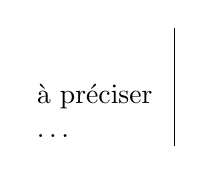
\begin{tikzpicture}
\node[align=left,anchor=east] at (-.15,.45) {à préciser\\$\ldots$};
\draw (0,0)--(0,1.5);
\end{tikzpicture}}}

\margin{\figure{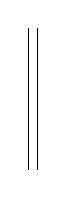
\begin{tikzpicture}\draw (0,0)--(0,1.8);\draw (.12,0)--(.12,1.8);\end{tikzpicture}}}
\uline{Remarque} On voit donc que la position de la filtration p.r. à la stratification ne peut aucunement donner un principe de classification \inserted{des déf.} infinitésimale en car. $p>0$ !
\mspage{17}
